\newcommand{\formula}{Formula}
\newcommand{\assignRoles}{Specify variable roles}

\def\arraystretch{0.35}
\newcommand{\tableSoftwareAnalysis}{
    \begin{table*}
        \footnotesize
        \caption{\textbf{Overview of the software tools included in our analysis.}\label{tableAnalysisOfTools}}
        \begin{small}
        \vspace*{-10pt}
        \begin{minipage}{\linewidth}
        \polish{Fit horizontal page margins. References column appears off.}
        Half of the tools
        are specialized for specific modeling use cases. Most tools
        use mathematical notation (T18--T20 (\yes*) even use
        mathematical notation in their GUIs).
        Most tools also provide a wide range
        of computational control although sometimes they require additional
        packages [T5, T13]. Tool specialization, organization,
        notation, and computational control focus analysts on model
        implementation details, sometimes at the expense of focusing on their conceptual
        hypotheses.
        \end{minipage}
        \end{small}
        
        \setlength{\tabcolsep}{4pt}
        \begin{tabular}{l>{\raggedright}p{0.3\linewidth}p{0.15\linewidth}p{0.15\linewidth}p{0.15\linewidth}p{0.2\linewidth}}
        \toprule
        ID & Tool name                                          & Specialized Scope    & Mathematical Notation        & Computational Control            & References                               \\                     
        \multicolumn{2}{l}{\textbf{R Packages}} \\
        \midrule\\
        T1 & MASS                                               & \no                  & \yes                         & \yes                             & ~\cite{mass}                                 \\                     
        T2 & brms                                               & \yes                 & \yes                         & \yes                             & ~\cite{burkner2017brms,brmsRef}                                 \\                     
        T3 & edgeR                                              & \yes                  & \yes                        & \yes                            & ~\cite{edgeROverview,edgeRUsersGuide}                                 \\                     
        T4 & glmmTMB                                            & \yes                 & \yes                         & \yes                             & ~\cite{glmmtmbPaper,glmmtmbRef}                                 \\                     
        T5 & glmnet                                             & \yes                 & \no                          & \yes (additional)                & ~\cite{glmnetRef,glmnetVignette}                                 \\                     
        T6 & lme4                                               & \yes                 & \yes                         & \yes                             & ~\cite{bates2014fittingLme4,bates2014lme4Ref}                                 \\                     
        T7 & MCMCglmm                                           & \yes                 & \yes                         & \yes                             & ~\cite{MCMCglmmPaper,MCMCglmmRef}                                 \\                     
        T8 & nlme                                               & \yes                 & \yes                         & \yes                             & ~\cite{nlmeRef}                                 \\                     
        T9 & RandomForest                                       & \yes                 & \yes                         & \yes (minimal)                   & ~\cite{randomForestR}                                 \\                     
        T10 & stats (core library)                              & \no                  & \yes                         & \yes                             & ~\cite{statsCoreRRef}                                 \\                     
        \multicolumn{2}{l}{\textbf{Python Packages}} \\                 
        \midrule\\                  
        T11 & Keras                                             & \yes                 & \no                          & \yes (minimal)                   & ~\cite{keras}                                 \\                     
        T12 & Scikit-learn                                      & \yes                 & \no                          & \yes                             & \cite{scikitRef,scikitPaper,scikitAPIPaper}                                 \\                                                                            
        T13 & Scipy (scipy.stats)                               & \no                  & \no                          & \yes (additional)                & ~\cite{scipy,scipyStats,scipyOptimize}                                 \\                     
        T14 & Statsmodels                                       & \no                  & \yes                         & \no                              & ~\cite{statsmodelsPaper,statsmodelsRef}                                 \\                                                                                  
        \multicolumn{2}{l}{\textbf{Suites, with DSLs for programming}} \\                   
        \midrule\\                  
        T15 & Matlab (Statistics and ML Toolbox)                & \no                  & \no                          & \yes                             & ~\cite{matlab,matlabStats}                                 \\                     
        T16 & SPSS                                              & \no                  & \yes                         & \yes                             & ~\cite{spss}                                 \\                                    
        T17 & Stata                                             & \no                  & \yes                         & \no                              & ~\cite{stata,stataRef,stataLang}                                 \\                     
        \multicolumn{2}{l}{\textbf{Suites, without programming}} \\                 
        \midrule\\                  
        T18 & GraphPrism                                        & \no                  & \yes *                       & \yes                             & ~\cite{graphPadUserGuide}                                 \\                                    
        T19 & JASP                                              & \no                  & \yes *                       & \no                              & ~\cite{jasp}                                 \\                                    
        T20 & JMP                                               & \no                  & \yes *                       & \no                              & ~\cite{jmp,jones2011jmp}                                 \\                                                                                  
        \bottomrule 
        \end{tabular}
        \vspace{-4mm}
        \end{table*}
        
}

\newcommand{\figureOverivew}{
    \begin{figure}[h]
        \centering
        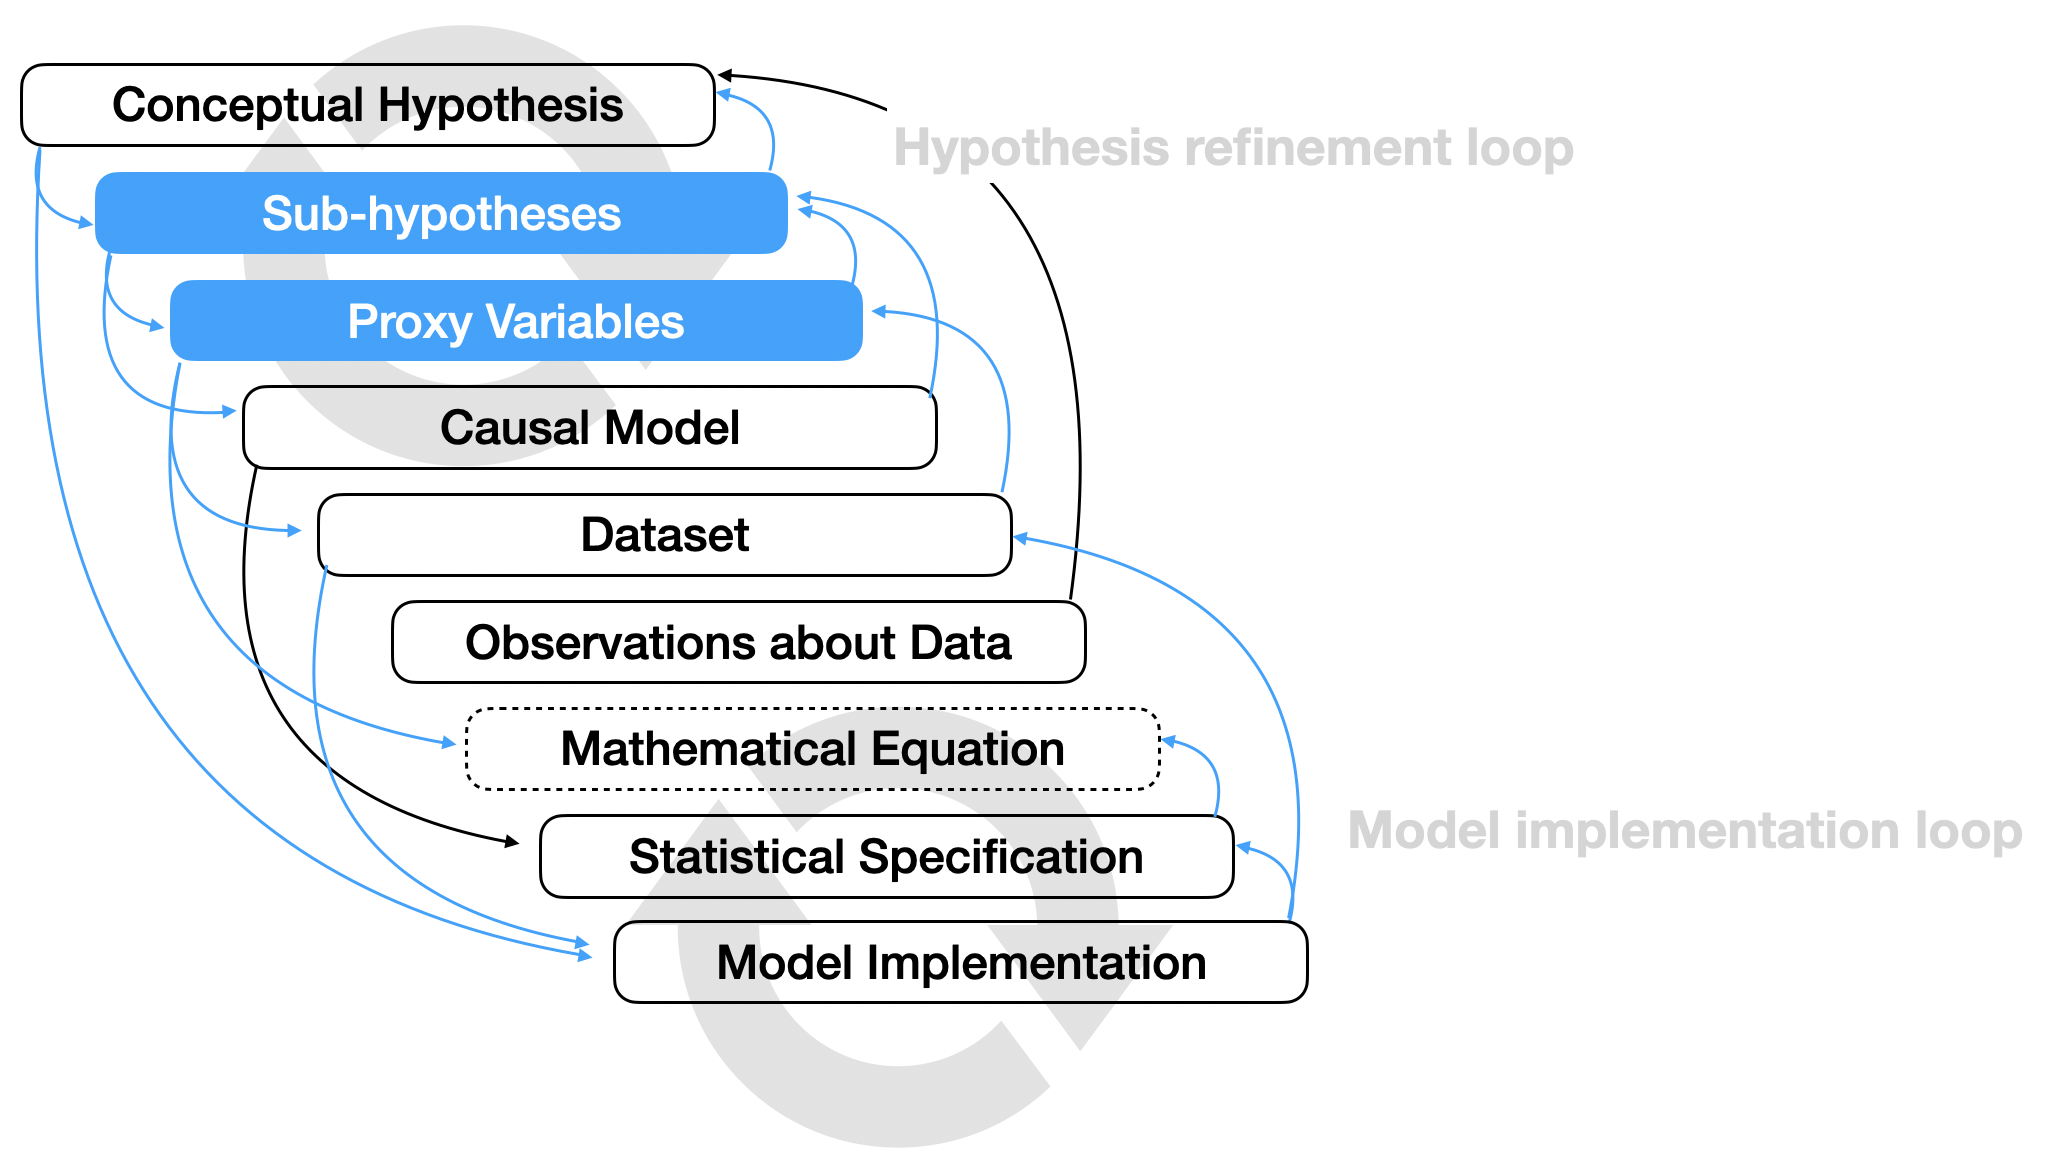
\includegraphics[width=.8\textwidth]{hypothesisFormalization/figures/overview_sept_17.png}
        \caption{\textbf{Definition and overview of the hypothesis formalization
        steps and process.}\label{figure:hypoFormOverview}}
        \begin{small}
        \begin{minipage}{\linewidth}
        Hypothesis formalization is a dual-search process of
        translating a \textbf{conceptual hypothesis} into a statistical
        \textbf{model implementation}.
        %
        Blue indicates steps and transitions that we identified.
        Black indicates steps and transitions discussed in prior work.
        ``Mathematical Equation'' (dashed box) was rarely an explicit step in
        our lab study but evident in our content analysis.
        Our findings (blue arrows) corroborate and subsume several of the transitions identified
        in prior work with greater granularity. When they do not, prior work's transitions are included in black.
        For example, analysts may operationalize a conceptual hypothesis as a causal model by first decomposing the conceptual hypothesis into sub-hypotheses and then identifying proxy variables to incorporate in a causal model (blue arrows above).
        Our definition of hypothesis formalization is a consequence of our synthesis of prior work, content analysis, lab study, and analysis of tools.
        % 
        Hypothesis formalization is a non-linear process.
        Analysts iterate over conceptual steps to refine their hypothesis in a
        \textit{hypothesis refinement loop}.
        Analysts also iterate over computational and implementation steps in a
        \textit{model implementation loop}.
        Data collection and data properties may also prompt conceptual revisions
        and influence statistical model implementation.
        %
        As analysts move toward model implementation, they increasingly rely on
        software tools, gain specificity, and create intermediate artifacts
        along the way (e.g., causal models, observations about data, etc.).
        % that help them satisfy conceptual, data, statistical, and computational constraints.
        \end{minipage}
        \end{small}
      \end{figure}
}

\newcommand{\figurePriorWorkCombined}{
    \begin{figure}[ht]
        \centering
        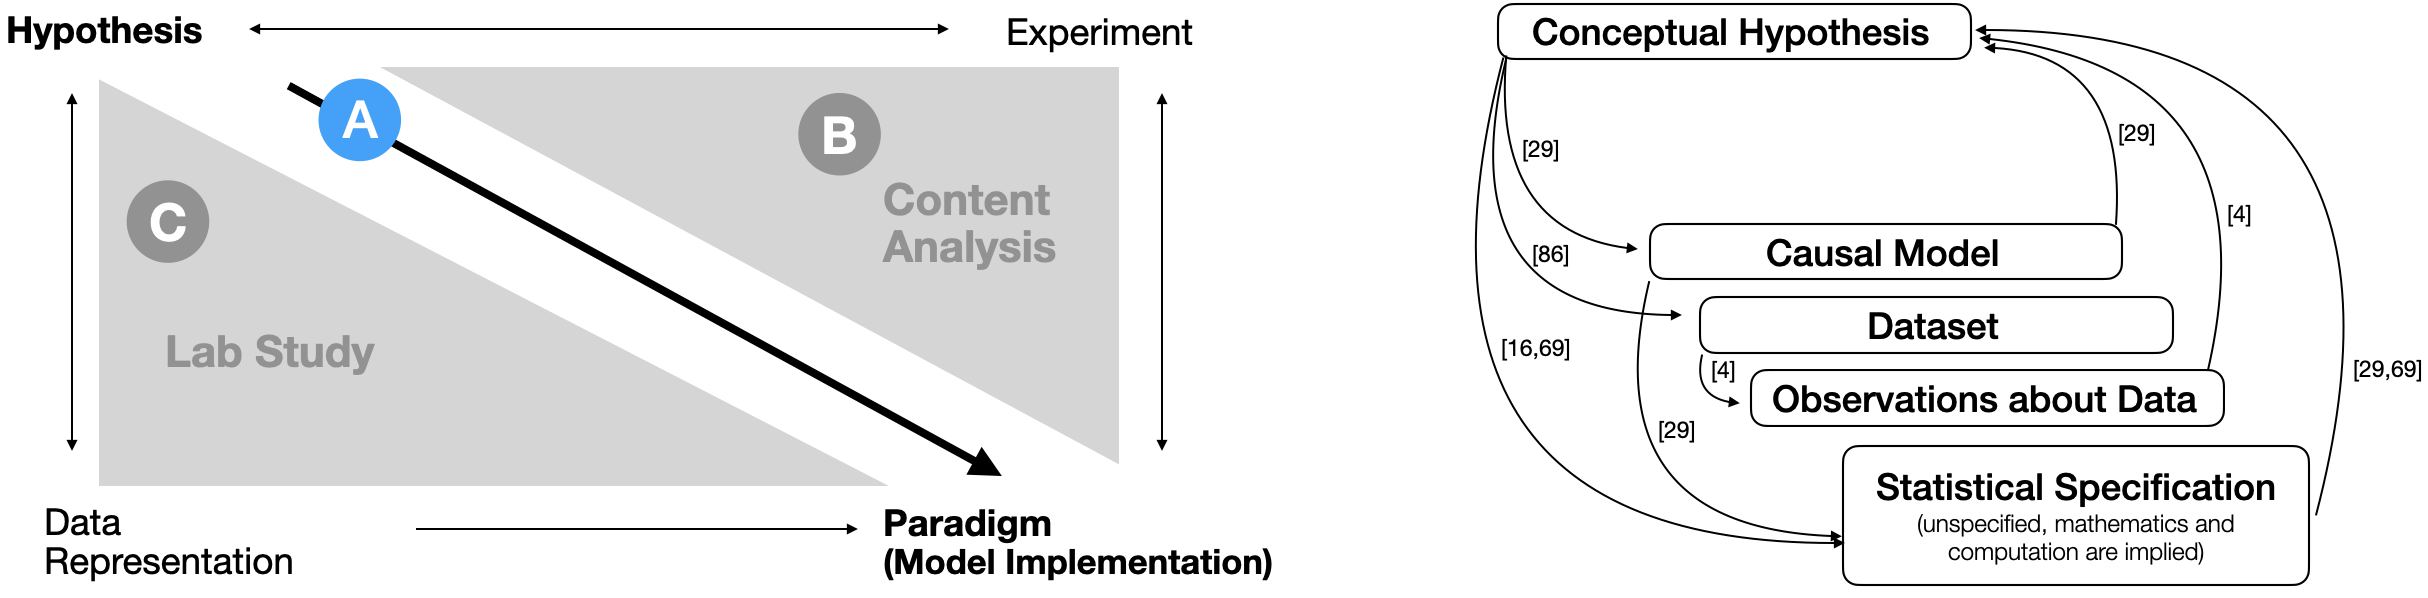
\includegraphics[width=0.8\textwidth]{hypothesisFormalization/figures/prior_work_combined_july_16_2021.png}
        \caption{\textbf{Relationship between hypothesis formalization and prior work.}\label{figure:priorWork}}
        \begin{small}
        \begin{minipage}{\linewidth}
            \polish{Make image content bigger to fill the horizontal space?; Update citations to match new citation style}

         \textit{Left:}
        Schunn and
        Klahr's four-space model of scientific
        discovery (stylized adaptation from  Figure 1 in~\cite{schunn1995FourSpace}),
        which includes unidirectional information flow
        from the hypothesis space to the paradigm space (which includes
        model implementation). Hypothesis formalization (A) is focused on a
        tighter integration and the information flow between hypothesis and paradigm spaces.
        Specifically, the information flow is bidirectional in hypothesis formalization.
        Our content analysis (B) and lab study (C) triangulate the four-space
        model to understand hypothesis formalization
        from complementary perspectives.
        \textit{Right:} Hypothesis formalization steps also identified in
        prior work on theories of
        sensemaking, statistical thinking, and data analysis workflows (citations included to the right of the arrows).
        Hypothesis formalization is finer grained and involves more iterations.
        While prior work broadly refers to mathematical equations,
        partial model specifications, and computationally tuned model
        implementations as statistical specifications, hypothesis formalization
        differentiates them. As a whole, this chapter provides empirical evidence for
        theorized loops between conceptual hypothesis and statistical
        specification (see Figure~\ref{figure:hypoFormOverview}).
        \end{minipage}
        \end{small}
        \vspace*{-15pt}
      \end{figure}
    % \begin{figure}
    %     \centering
    %     \begin{subfigure}{.5\textwidth}
    %         \centering
    %         \includegraphics[width=.5\textwidth]{hypothesisFormalization/figures/methods_overview.png}
    %         \caption{A subfigure}
    %         \label{fig:sub1}
    %     \end{subfigure}%
    %     \begin{subfigure}{.5\textwidth}
    %         \centering
    %         \includegraphics[width=.5\textwidth]{hypothesisFormalization/figures/prior_work_sept_11.png}
    %         \caption{A subfigure}
    %         \label{fig:sub2}
    %     \end{subfigure}
    %     \caption{A figure with two subfigures}
    %     \label{fig:test}
    % \end{figure}
}

\newcommand{\figureLabStudyStatSpec}{
    \begin{figure*}[tb]
        \centering
        \begin{minipage}{0.45\textwidth}
            \centering
            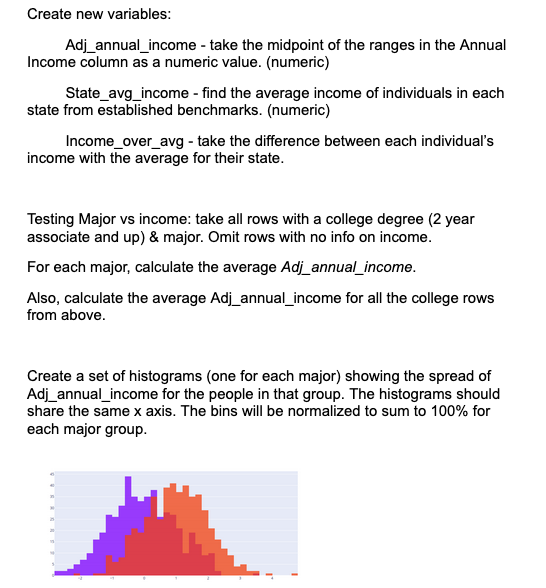
\includegraphics[width=0.9\textwidth]{hypothesisFormalization/figures/A11_SS_1.png} % first figure itself
        \end{minipage}\hfill
        \begin{minipage}{0.45\textwidth}
            \centering
            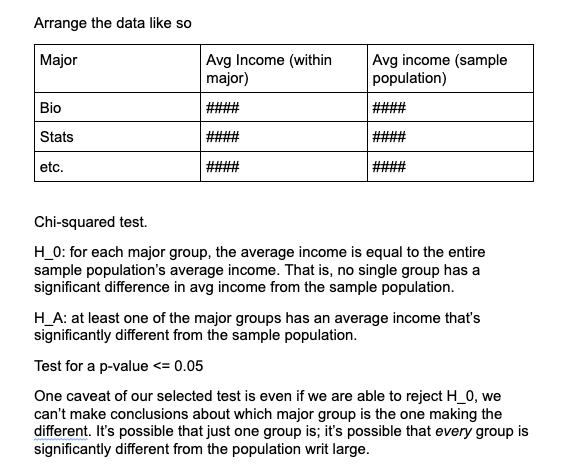
\includegraphics[width=0.9\textwidth]{hypothesisFormalization/figures/A11_SS_2.png} % second figure itself
        \end{minipage}
        \caption{\textbf{Sample statistical specification from analyst D8 in the lab study.}\label{figure:labStudyStatSpec}}
            \begin{small}
            \begin{minipage}{\linewidth}
            The lab study tasked analysts
            to specify their statistical models without
            considering implementation. 
            We expected analysts would represent
            their statistical models using statistical test names or mathematical equations. 
            %their statistical models mathematically. 
            Instead, most analysts specified statistical procedures for performing statistical models 
            using todo lists and summaries of steps,
            which sometimes included mentions of software tools, showing that
            implementation was an important consideration and
            that tool familiarity may limit which statistical models
            analysts consider and implement.
            Data worker D8 specified their model through a combination of statistical test names (e.g., Chi-squared test) and a list (split across two pages) of detailed steps
            involved in creating new variables, cleaning and wrangling data,
            visualizing data, and testing their hypothesis. 
            \end{minipage}
            \end{small}
    \end{figure*}
}

\newcommand{\figureExampleReorderableMatrix}{
    \begin{figure}
        \centering
        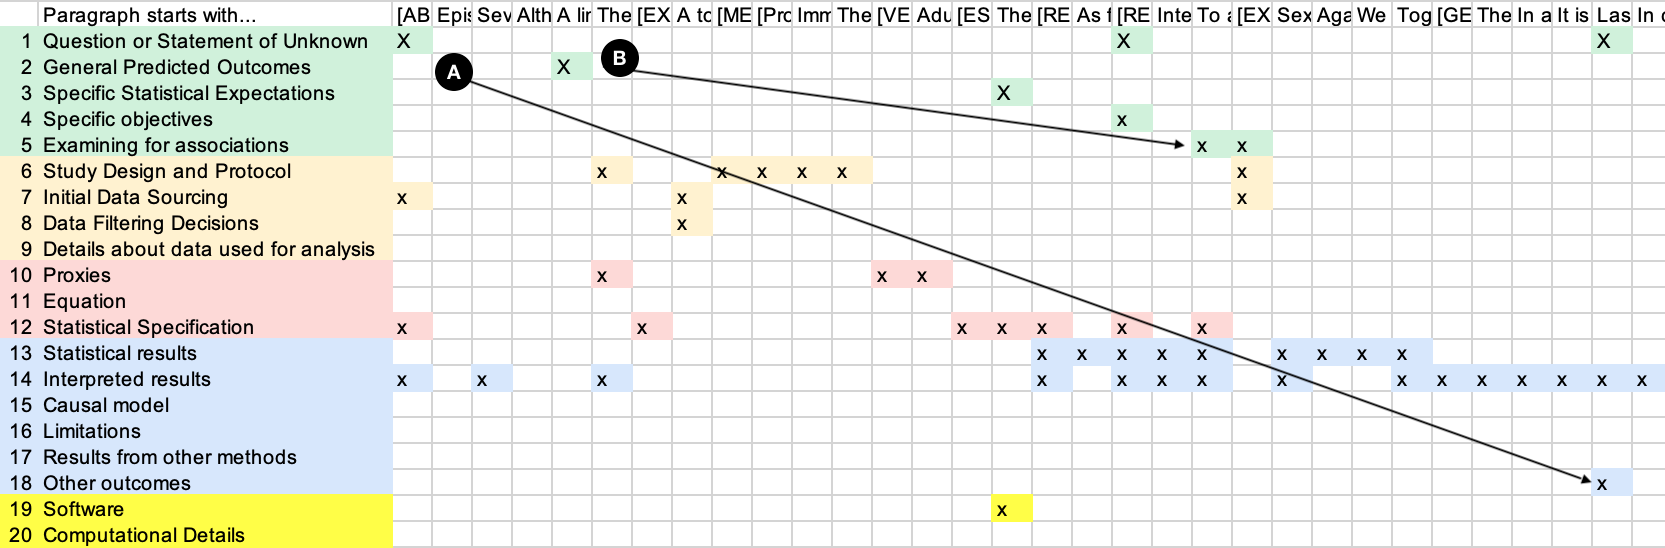
\includegraphics[width=0.95\textwidth]{hypothesisFormalization/figures/ps9_reorderableMatrixLabeled.png}
        \caption{\textbf{Example reorderable matrix for Ngo et al.'s 
        ``Development of holistic episodic recollection'' published in \textit{Psychological Science} (2019)~\cite{PS9} from the formative content analysis.}\label{figure:exampleReorderableMatrix}}
        \begin{small}
            \begin{minipage}{\linewidth}
            %
            We visualized each paper in our sample as a ``reorderable
            matrix''~\cite{bertin2011graphics} to aid in detecting patterns in
            papers' structure and content that could indicate how researchers
            formalized their hypotheses. The rows represent the codes in our
            \codebook, colored according to the five broad categories of codes:
            research goals (rows 1-5, green), sample information (rows 6-9,
            orange), statistical analysis details (rows 10-12, red), reporting
            of results (rows 13-18, blue), and computational details (rows
            19-20, bright yellow). The columns are the paragraphs, which are indexed by
            their first sentences, ordered left to right. In a paragraph's
            column, there is an ``X'' for each code the paragraph received.
            Paragraphs have multiple codes if they contain multiple types of
            information. 
            %
            Among the ten visual patterns we noticed across our sample and
            subsequently looked for in each paper, two stand out in this paper.
            (A) As the paper progresses (visually moving left to right), the
            paper's focus shifts from research goals to sample information to
            statistical analysis to results, as indicated by the arrow labeled
            A. Largely expected, this pattern helps to validate our coding
            method. Also, there is only one paragraph that discusses statistical
            software. (B) Researchers discuss research goals and questions
            throughout the paper. Interestingly, in the middle of the paper,
            when the researchers discuss their goals in greater detail, the
            researchers discuss them in increasing specificity, as indicated by
            the arrow labeled B. We were able to detect this pattern across
            papers by iterating on how to order the research goal codes (rows
            1-5, green). The final order lists codes in increasing specificity
            from top (row 1) to bottom (row 5). Pattern B suggests that
            researchers refine their hypotheses during hypothesis formalization,
            which may involve specifying proxies and statistical methods.
            %
            \autoref{chapter:appHypoForm} discusses additional patterns in this paper
            and across our entire sample. 
            \end{minipage}
        \end{small}
    \end{figure}
}